\documentclass[a4paper,11pt]{article}
\usepackage[utf8]{inputenc}
\usepackage[spanish]{babel}
\usepackage[affil-it]{authblk}
\usepackage{enumerate}
\usepackage{graphicx}
\usepackage{hyperref}
\usepackage{amsmath}
\usepackage{amssymb}
\usepackage{cancel}
\usepackage[usenames, dvipsnames]{color}
\usepackage{tikz}
\usepackage[labelfont=bf]{caption}
\usepackage{subcaption} %Multiple images
\usepackage{multicol} % Multiple columns
\usepackage{float}
\usepackage{cleveref}
\usepackage{relsize} % bigger math symbols
\usepackage[margin=1.1in]{geometry}
\usepackage[titletoc,toc,title]{appendix}
\usepackage{enumitem}
\usepackage{etoolbox}
\usepackage{mdframed} %frame theorems
\usetikzlibrary{calc}
\numberwithin{equation}{section}

% Footnotes with symbols

\makeatletter
\def\@fnsymbol#1{\ensuremath{\ifcase#1\or \dagger\or \ddagger\or
   \mathsection\or \mathparagraph\or \|\or **\or \dagger\dagger
   \or \ddagger\ddagger \else\@ctrerr\fi}}
\makeatother

\renewcommand{\thefootnote}{\fnsymbol{footnote}}

% Cool letters 
%Filename:      Typocaps.fd
%Created by:    MLO
%Creation date: 2003/04/02

% This file should be put in a TeX input directory

\ProvidesFile{Typocaps.fd}
   [2003/04/02 Font definition file for U/Typocaps]

\DeclareFontFamily{U}{Typocaps}{}

\DeclareFontShape{U}{Typocaps}{xl}{n}{
   <-> Typocaps
}{}

\endinput


% Footer
\usepackage{fancyhdr}
\pagestyle{fancy}
\fancyhf{}
\cfoot{\fontsize{15pt}{15pt}\usefont{U}{Typocaps}{xl}{n} 
gigantium humeris insidentes}

% Big Pictures
\usepackage[export]{adjustbox}

% Enviroment for theorems
\newmdtheoremenv[frametitle=Teorema]{theo}{Theorem}

% Circled words
\newcommand{\circled}[2][]{%
  \tikz[baseline=(char.base)]{%
    \node[shape = circle, draw, inner sep = 1pt]
    (char) {\phantom{\ifblank{#1}{#2}{#1}}};%
    \node at (char.center) {\makebox[0pt][c]{#2}};}}
\robustify{\circled}

%Appendices in spanish
\renewcommand{\appendixname}{Ap\'endices}
\renewcommand{\appendixtocname}{Ap\'endices}
\renewcommand{\appendixpagename}{Ap\'endices}

%Zero delimiter
\newcommand{\zerodel}{.\kern-\nulldelimiterspace}

%Columns separation
\setlength{\columnsep}{1cm}

%Indentation
\setlength{\parindent}{0ex}

%Multiple References

\crefrangelabelformat{equation}{(#3#1#4--#5\crefstripprefix{#1}{#2}#6)}

\usepackage{xparse}

%Boxes

\newcommand*{\boxcolor}{blue}
\makeatletter
\renewcommand{\boxed}[1]{\textcolor{\boxcolor}{%
\tikz[baseline={([yshift=-1ex]current bounding box.center)}] \node [rectangle, minimum width=1ex,rounded corners,draw] {\normalcolor\m@th$\displaystyle#1$};}}
 \makeatother

%Constantes
\newcommand{\euler}{\mathrm{e}}
\newcommand{\im}{i}

%Lemas, teoremas, definiciones y pruebas
\newcommand{\definicion}{\textbf{Definición: }}
\newcommand{\lema}{\textbf{Lema: }}
\newcommand{\teorema}{\textbf{Teorema: }}
\newcommand{\prueba}{\textbf{Prueba: }}
\newcommand{\proposicion}{\textbf{Proposición: }}
\newcommand{\corolario}{\textbf{Corolario: }}

% Definición de las secciones y su numeración

\makeatletter
\def\@seccntformat#1{%
  \expandafter\ifx\csname c@#1\endcsname\c@section\else
  \csname the#1\endcsname\quad
  \fi}
\makeatother

\begin{document}

\begin{titlepage}
\thispagestyle{fancy}

\newcommand{\HRule}{\rule{\linewidth}{0.5mm}} % Defines a new command for the horizontal lines, change thickness here

\center % Center everything on the page
 
%----------------------------------------------------------------------------------------
%	HEADING SECTIONS
%----------------------------------------------------------------------------------------

\textsc{\LARGE Universidad Nacional Autónoma de México}\\[0.3cm] % Name of your university/college

%----------------------------------------------------------------------------------------
%	LOGO SECTION
%----------------------------------------------------------------------------------------


\includegraphics[scale=0.17]{unam}

%----------------------------------------------------------------------------------------
%	SUBHEADING SECTIONS
%----------------------------------------------------------------------------------------

\textsc{\Large Electrodinámica Clásica}\\[0.3cm] % Major heading such as course name
\textsc{\large Semestre 2016-II}\\[0.3cm] % Minor heading such as course title
\textsc{\large 17 de marzo de 2016}\\ % Minor heading such as course title

%----------------------------------------------------------------------------------------
%	TITLE SECTION
%----------------------------------------------------------------------------------------

\HRule \\[0.1cm]
{ \huge \bfseries Tarea \# 5. \\ Ecuaciones de Maxwell, 
electromagnetismo macroscópico y leyes de conservación.}\\ % Title of your document
\HRule \\[0.1cm]
 
%----------------------------------------------------------------------------------------
%	AUTHOR SECTION
%----------------------------------------------------------------------------------------
\setcounter{footnote}{0}
\center
\large
\emph{Autor:} \\ % Your name
\Large Favio \textsc{Vázquez}\footnote[1]{\href{mailto:favio.vazquez@correo.nucleares.unam.mx}{favio.vazquez@correo.nucleares.unam.mx}}
\\[0.7cm]
%----------------------------------------------------------------------------------------
%	COOL IMAGE SECTION
%----------------------------------------------------------------------------------------

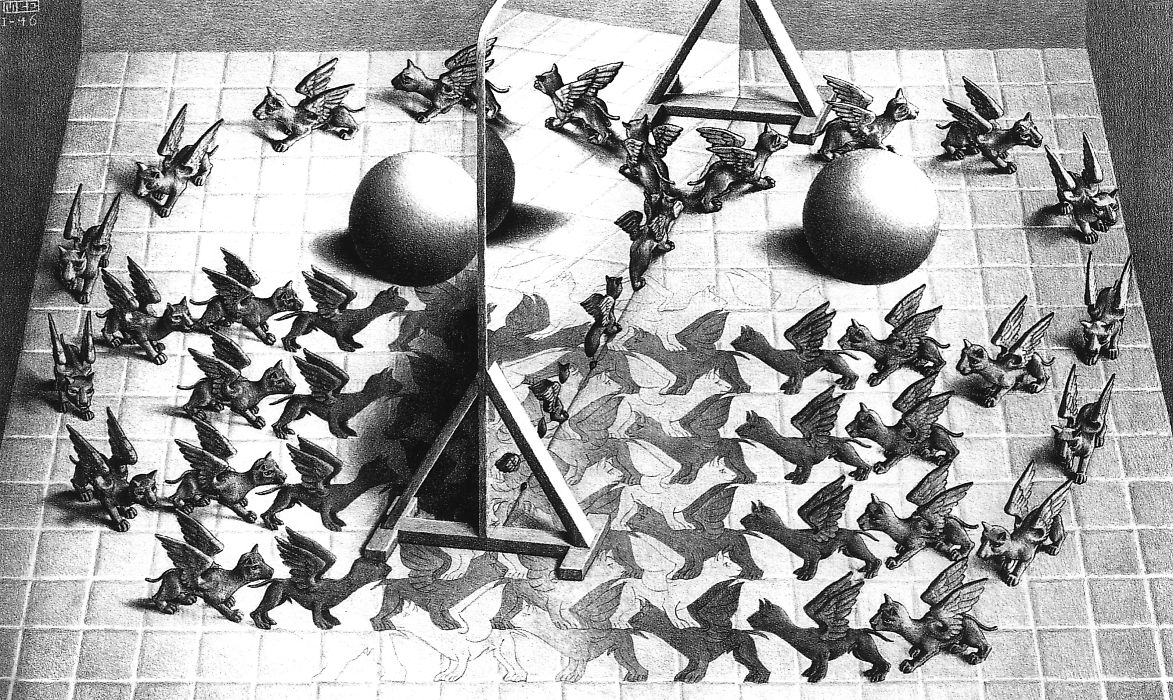
\includegraphics[scale=1.55]{escherEspejo2D}

%----------------------------------------------------------------------------------------

\vfill % Fill the rest of the page with whitespace

\end{titlepage}

% ---------------------------------------------------------------------------------------
%         HEADER
%----------------------------------------------------------------------------------------

\fancyhead[L]{Favio Vázquez}
\fancyhead[R]{\thepage}

%----------------------------------------------------------------------------------------
\setcounter{footnote}{0}
\renewcommand*{\thefootnote}{\arabic{footnote}}
%----------------------------------------------------------------------------------------

%----------------------------------------------------------------------------------------
%%			BEGIN DOCUMENT
%----------------------------------------------------------------------------------------

\section{Problema 1. Problema 6.8 de Classical Electromagnetic Radiation
de Jackson \cite{jackson}.}

Una esfera de constante dieléctrica constante $\epsilon$ y radio $a$ está situada 
en el origen. Hay un campo eléctrico $E_0$ uniforme aplicado en la dirección $x$. 
La esfera rota con una velocidad angular $\omega$ sobre el eje $z$. Muestre que 
hay un campo magnético $\mathbf{H} = - \mathbf{\nabla} \Phi_M$, donde 

$$
\Phi_M = \frac{3}{5}\left(\frac{\epsilon - \epsilon_0}{\epsilon + 2\epsilon_0}\right)
\epsilon_0E_0\omega\left(\frac{a}{r_>}\right)^5\cdot xz,
$$

donde $r_>$ es el más grande de $r$ y $a$. El movimiento es no relativista. Puede 
utilizar los resultados de la sección $4.4$ para la esfera dieléctrica en un campo 
aplicado.

\vspace{.3cm}

\underline{Solución:} \vspace{.3cm}

La idea básica que nos ayudará a solucionar este problema, fue lo que se vio en 
clase y en la sección 4.4 de Jackson \cite{jackson}, y es que un campo uniforme
$E_0$ aplicado a la esfera la polariza, induciendo una carga superficial de 
polarización (o ligada) sobre la misma, la cual se convierte en corriente de 
polarización (o ligada) debido a la rotación de la esfera. Y como se vio en el 
capítulo 6 de Jackson \cite{jackson} estas corrientes dan lugar a campos 
magnéticos.

\vspace{.3cm}

Para obtener el potencial magnético que nos pide el problema, utilizaremos la expresión 
indicada en la ecuación (5.100) de Jackson \cite{jackson}, para el caso en que 
la magnetización sobre el volumen de integración es constante y por lo tanto 
se cancela el primer término de esta ecuación y nos queda 

\begin{equation}
 \Phi_M = \frac{1}{4\pi} \oint_s \frac{\sigma_M}{|\mathbf{x} - \mathbf{x'}|}da',
 \label{eq:potencialMagnetico}
\end{equation}

y por lo tanto necesitamos una expresión para la densidad superficial de carga magnética 
$\sigma_M$, y ya que esta depende del momento magnético total $\mathbf{M}$ debemos
calcularlo. Esto  lo haremos calculando primero la densidad de corriente superficial
 $\mathbf{J}_M$ inducida en la esfera a partir de su polarización, tomando en cuenta la rotación
de la misma.

\vspace{.3cm}

De la sección 4.4 sabemos que la carga superficial inducida en la esfera 
será\footnote{Ver ecuación (4.58) de Jackson \cite{jackson}.}, en coordenadas 
cartesianas 

\begin{equation}
 \sigma_{pol} \equiv \sigma =  3 \left(\frac{\epsilon - \epsilon_0}{\epsilon + 2\epsilon_0}
 \right)\epsilon_0E_0 \frac{x}{a}.
\end{equation}

Ahora debido a que esta densidad de carga está girando en la superficie de la esfera 
de radio $a$ a una velocidad angular $\omega$, utilizando\footnote{Ver página 187 de 
Jackson \cite{jackson}.}

\begin{equation}
 \mathbf{J}_M = \sigma \mathbf{v},
\end{equation}

el hecho de que $\mathbf{v} = \pmb{\omega} \times \mathbf{r}$ y que la velocidad 
angular puede escribirse como $\pmb{\omega} = \omega \hat{z}$ y $\mathbf{r} = a
\hat{r}$ obtenemos 

\begin{equation}
 \mathbf{J}_M = \sigma (\omega \hat{z}) \times (a\hat{r}),
\end{equation}

\begin{equation}
 \therefore \mathbf{J}_M = \sigma \omega a \sen{\theta} \hat{\phi},
\end{equation}

donde hemos utilizado que en coordenadas esféricas $\hat{z} \times \hat{r} = \hat{\phi}$, 
y sustituyendo la expresión para la densidad superficial obtenemos

\begin{equation}
 \mathbf{J}_M = 3 \left(\frac{\epsilon - \epsilon_0}{\epsilon + 2\epsilon_0}
 \right)\epsilon_0E_0 x \sen{\theta} \hat{\phi}.
\end{equation}

Ya que obtuvimos la densidad de corriente superficial podemos obtener el momento 
magnético total con\footnote{Ver ecuación (5.79) de Jackson \cite{jackson}.}

\begin{equation}
  \mathbf{J}_M = \mathbf{M} \times \hat{r},
\end{equation}

y debido que el momento magnético estará dirigido exclusivamente hacia el lado positivo 
del eje $z$, tenemos 

\begin{equation}
  \mathbf{J}_M = (M\hat{z}) \times \hat{r},
\end{equation}

ahora utilizando la definición del producto vectorial, las propiedades de los vectores 
unitarios en coordenadas esféricas y la expresión que obtuvimos para 
$ \mathbf{J}_M$ esta ecuación se puede escribir como 

\begin{equation}
 M \sen{\theta}\hat{\phi} =  3\left(\frac{\epsilon - \epsilon_0}{\epsilon + 2\epsilon_0}
 \right)\epsilon_0E_0 x \sen{\theta} \hat{\phi},
\end{equation}

y resolviendo para el momento magnético obtenemos 

\begin{equation}
 \mathbf{M} =  3\left(\frac{\epsilon - \epsilon_0}{\epsilon + 2\epsilon_0}
 \right)\epsilon_0E_0 x \hat{z}.
\end{equation}

Lo único que nos falta para poder utilizar la ecuación \eqref{eq:potencialMagnetico}
es obtener una expresión para la densidad  densidad superficial de carga magnética, lo 
cual podemos hacer utilizando la ecuación (5.99) de Jackson \cite{jackson}, 

\begin{equation}
 \sigma_M = \mathbf{n} \times \mathbf{M},
\end{equation}

que en nuestro caso puede escribirse como 

\begin{equation}
 \sigma_M = \hat{r} \times \mathbf{M},
\end{equation}

y sustituyendo la expresión que obtuvimos para el momento magnético nos queda

\begin{equation}
 \sigma_M = 3\left(\frac{\epsilon - \epsilon_0}{\epsilon + 2\epsilon_0}
 \right)\epsilon_0E_0 \frac{\omega}{a} xz.
\end{equation}

Estamos ahora en posición para utilizar la ecuación \eqref{eq:potencialMagnetico} y 
calcular el potencial magnético; pero, para expresarlo en la notación que utiliza 
el texto conviene primero expandir $1/|\mathbf{x} - \mathbf{x}'|$ en esféricos 
armónicos, entonces\footnote{Ver ecuación (3.70) de Jackson \cite{jackson}.}

\begin{equation}
 \frac{1}{|\mathbf{x} - \mathbf{x}'|} = 4\pi \sum_{l=0}^\infty \sum_{m=-l}^l 
 \frac{1}{2l+1}\frac{r_<^l}{r_>^{l+1}}Y_{lm}^*(\theta',\phi')Y_{lm}(\theta,\phi).
\end{equation}

Entonces \eqref{eq:potencialMagnetico} se escribe como\footnote{Donde hemos utilizado 
las expresiones para $x$ y $z$ en coordenadas esféricas.}

\begin{align*}
 \Phi_M = &3\left(\frac{\epsilon - \epsilon_0}{\epsilon + 2\epsilon_0}
 \right)\epsilon_0E_0 \frac{\omega}{a}\left[ \int_0^{\pi}\int_0^{2\pi} a^2\sen{\theta}'
 \cos{\theta}'\cos{\phi}'\right\zerodel  \\
 &\left\zerodel\sum_{l=0}^\infty \sum_{m=-l}^l 
 \frac{1}{2l+1}\frac{r_<^l}{r_>^{l+1}}Y_{lm}^*(\theta',\phi')Y_{lm}(\theta,\phi)
 a^2\sen{\theta}'d\theta'd\phi'\right],
\end{align*}

que podemos escribir como 

\begin{align*}
 \Phi_M = &3\left(\frac{\epsilon - \epsilon_0}{\epsilon + 2\epsilon_0}
 \right)\epsilon_0E_0 \omega a^3 \sum_{l=0}^\infty \sum_{m=-l}^l 
 \frac{1}{2l+1}\frac{r_<^l}{r_>^{l+1}}Y_{lm}(\theta',\phi')\left[ \int_0^{\pi}\int_0^{2\pi} \sen{\theta}'
 \cos{\theta}'\cos{\phi}'\right\zerodel \\
 &\left\zerodel Y_{lm}^*(\theta,\phi)
 a^2\sen{\theta}'d\theta'd\phi' \frac{}{} \right],
\end{align*}

Y usando la relación 

\begin{equation}
 \sin{\theta}'\cos{\theta}'\cos{\phi}' = \sqrt{\frac{2\pi}{15}}(Y_{2,-1} - Y_{2,1}),
\end{equation}

obtenemos 

\begin{align*}
 \Phi_M = &3\left(\frac{\epsilon - \epsilon_0}{\epsilon + 2\epsilon_0}
 \right)\epsilon_0E_0 \omega a^3 \sum_{l=0}^\infty \sum_{m=-l}^l 
 \frac{1}{2l+1}\frac{r_<^l}{r_>^{l+1}}Y_{lm}(\theta',\phi')\left[ \int_0^{\pi}\int_0^{2\pi} 
 \sqrt{\frac{2\pi}{15}}(Y_{2,-1} - Y_{2,1})\right\zerodel \\
 &\left\zerodel Y_{lm}^*(\theta,\phi)
 a^2\sen{\theta}'d\theta'd\phi' \frac{}{} \right],
\end{align*}

usando las propiedades de los armónicos esféricos podemos integrar y obtener 

\begin{equation}
  \Phi_M = 3\left(\frac{\epsilon - \epsilon_0}{\epsilon + 2\epsilon_0}
 \right)\epsilon_0E_0 \omega a^3 \sum_{l=0}^\infty \sum_{m=-l}^l 
 \frac{1}{2l+1}\frac{r_<^l}{r_>^{l+1}}Y_{lm}(\theta',\phi')\sqrt{\frac{2\pi}{15}}
 [\delta_{l,2}\delta_{m,-1} - \delta_{1,2}\delta_{m,1}],
\end{equation}

que siguiendo los resultados de la sección 3.9 de Jackson \cite{jackson} escribimos 
como

\begin{equation}
 \Phi_M = \frac{3}{5}\left(\frac{\epsilon - \epsilon_0}{\epsilon + 2\epsilon_0}
 \right)\epsilon_0E_0 \omega a^3\frac{r_<^2}{r_>^3}\frac{xz}{r}.
\end{equation}

Entonces tenemos dos casos, si $r < a$ se cancelarán las contribuciones de las $r^2$ 
y la $a^3$ con $r^3$ obtenemos 

\begin{equation}
 \Phi_M = \frac{3}{5}\left(\frac{\epsilon - \epsilon_0}{\epsilon + 2\epsilon_0}
 \right)\epsilon_0E_0 \omega xz,
\end{equation}

y si $r>a$, 

\begin{equation}
 \Phi_M = \frac{3}{5}\left(\frac{\epsilon - \epsilon_0}{\epsilon + 2\epsilon_0}
 \right)\epsilon_0E_0 \omega \frac{a^5}{r_5}xz.
\end{equation}

Si ahora combinamos estos resultados obtenemos 

\begin{equation}
\boxed{\Phi_M = \frac{3}{5}\left(\frac{\epsilon - \epsilon_0}{\epsilon + 2\epsilon_0}\right)
\epsilon_0E_0\omega\left(\frac{a}{r_>}\right)^5\cdot xz}.
\end{equation}

\hspace{10cm}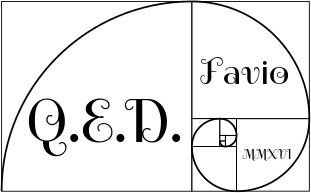
\includegraphics[scale=0.25]{logoQED}

\newpage

\section{Problema 2. Problema 6.9 de Classical Electromagnetic Radiation
de Jackson \cite{jackson}.}

Discuta la conservación de la energía y el impulso lineal para un sistema macroscópico 
de fuentes y campos electromagnéticos en un medio uniforme e isotrópico, descrito 
por una permitividad $\epsilon$ y una permeabilidad $\mu$. Muestre en un cálculo 
simple que la densidad de energía, el vector de Poynting, la densidad de campo-impulso, 
y el tensor de esfuerzo de Maxwell están dados por las expresiones de Minkowski,

\begin{align*}
u &= \frac{1}{2}(\epsilon E^2 + \mu H^2), \\
\mathbf{S} &= \mathbf{E} \times \mathbf{H}, \\
\mathbf{g} &= \mu\epsilon \mathbf{E} \times \mathbf{H}, \\
T_{ij} &= [\epsilon E_iE_j + \mu H_iH_j - \frac{1}{2}\delta_{ij}(\epsilon E^2 + \mu H^2)].
\end{align*}

¿Qué modificaciones surgen si $\epsilon$ y $\mu$ son funciones de la posición?

\vspace{.3cm}

\underline{Solución:} \vspace{.3cm}

\begin{mdframed}[linewidth=2]
\textbf{Nota}: Los resultados solicitados por el problema se encuentran adentro 
de cajas (marcos). Todas las demás ecuaciones son solamente necesarias para 
su deducción y para que la demostración sea completa y autosuficiente.
\end{mdframed}

Comencemos con la ecuación de la fuerza de Lorentz 

\begin{equation}
 \mathbf{F} = q(\mathbf{E} + \mathbf{v} \times \mathbf{B}),
\end{equation}

si multiplicamos ambos lados de esta ecuación por la velocidad obtenemos 

\begin{equation}
 \mathbf{F}\cdot d\mathbf{l} = q(\mathbf{E} + \mathbf{v} \times \mathbf{B})\cdot 
 \mathbf{v}dt,
\end{equation}

y por las propiedades del producto vectorial esta ecuación se convierte en 

\begin{equation}
 \mathbf{F}\cdot d\mathbf{l} = q\mathbf{E}\cdot \mathbf{v}dt,
\end{equation}

En términos de densidades de carga y corrientes\footnote{$q \rightarrow \rho d\tau$ 
y $\rho\mathbf{v} \rightarrow \mathbf{J}$. Ver página 357 de Griffiths \cite{griffiths}.} 
esta ecuación puede escribirse como\footnote{Ver ecuación (8.6) de Griffiths \cite{griffiths}.}
el trabajo que es hecho sobre todas las cargas en un volumen $V$ 

\begin{equation}
 \frac{dW}{dt} = \int_V (\mathbf{E} \cdot \mathbf{J}) d\tau.
\end{equation}

Ahora para un sistema macroscópicos de fuentes y campos electromagnéticos en 
un medio uniforme e isotrópico, solo nos interesa el trabajo hecho sobre las cargas y 
corrientes libres, entonces esta ecuación se convierte en\footnote{$l$ se refiere 
a ``libre''.}

\begin{equation}
 \frac{dW}{dt} = \int_V (\mathbf{E} \cdot \mathbf{J}_l) d\tau.
 \label{eq:trabajoMateriales}
\end{equation}

Ahora de la ley de Ampère-Maxwell para medios 

\begin{equation}
 \pmb{\nabla} \times \mathbf{H} = \mathbf{J}_l + \frac{\partial \mathbf{D}}{\partial t},
\label{eq:amperemaxwell}
\end{equation}

vemos que 

\begin{equation}
 \mathbf{J}_l = \pmb{\nabla} \times \mathbf{H} - \frac{\partial \mathbf{D}}{\partial t},
\end{equation}

y tomando el producto punto en ambos lados del campo eléctrico obtenemos 

\begin{equation}
 \mathbf{E} \cdot \mathbf{J}_l  = \mathbf{E} \cdot (\pmb{\nabla} \times \mathbf{H}) - 
  \mathbf{E} \cdot \frac{\partial \mathbf{D}}{\partial t}.
\end{equation}

Ahora utilizando propiedades de productos vectoriales tenemos que 

\begin{equation}
 \mathbf{\nabla} \cdot (\mathbf{E} \times \mathbf{H}) = \mathbf{H} \cdot 
 (\mathbf{\nabla} \times \mathbf{E}) - \mathbf{E}\cdot (\mathbf{\nabla} \times 
 \mathbf{H}),
\end{equation}

y recordando que 

\begin{equation}
 \mathbf{\nabla} \times \mathbf{E} = - \frac{\mathbf{B}}{\partial t},
\end{equation}

obtenemos 

\begin{equation}
  \mathbf{E}\cdot (\mathbf{\nabla} \times 
 \mathbf{H}) = - \mathbf{H}\cdot \frac{\mathbf{B}}{\partial t} - 
 \mathbf{\nabla} \cdot (\mathbf{E} \times \mathbf{H}).
\end{equation}

Y podemos reescribir \eqref{eq:amperemaxwell} como 

\begin{equation}
 \mathbf{E} \cdot \mathbf{J}_l = - \mathbf{H}\cdot \frac{\mathbf{B}}{\partial t}
 - \frac{\partial \mathbf{D}}{\partial t} - \mathbf{\nabla} \cdot (\mathbf{E} \times \mathbf{H}),
\end{equation}

sustituyendo esta ecuación en \eqref{eq:trabajoMateriales} obtenemos\footnote{Donde 
hemos usado el teorema de Gauss.}

\begin{equation}
 \frac{dW}{dt} = - \int_V \left(\mathbf{E} \cdot \frac{\partial \mathbf{D}}{\partial 
 t} + \mathbf{H}\cdot\frac{\partial \mathbf{B}}{\partial t} \right) - 
 \oint_s (\mathbf{E} \times \mathbf{H})\cdot d\mathbf{a}.
 \label{eq:consEnergiaMateriales}
\end{equation}

Este es el teorema de Poynting para los campos electromagnéticos en materiales. De 
forma análoga al caso de campos electromagnéticos en el vacío podemos identificar 
el vector de Poynting como (segundo término del lado derecho 
de \eqref{eq:consEnergiaMateriales}) 

\begin{equation}
 \boxed{\mathbf{S} = \mathbf{E} \times \mathbf{H}},
\end{equation}

el cual representa la potencia por unidad de área transportada por los campos. Y 
también podemos ver que la tasa de cambio de la densidad de energía de 
electromagnética es (primer término del lado derecho 
de \eqref{eq:consEnergiaMateriales})

\begin{equation}
 \frac{\partial u}{\partial t} = \mathbf{E} \cdot \frac{\partial \mathbf{D}}{\partial 
 t} + \mathbf{H}\cdot\frac{\partial \mathbf{B}}{\partial t},
\end{equation}

ahora ya que tratamos con un medio uniforme e isotrópico descrito por una permitividad 
$\epsilon$ y una permeabilidad $\mu$ tenemos que 

\begin{equation}
 \mathbf{D} = \epsilon\mathbf{E} \qquad \quad \mathbf{B} = \mu\mathbf{H}, 
\end{equation}

y por lo tanto

\begin{equation}
 \frac{\partial u}{\partial t} = \epsilon\mathbf{E} \cdot \frac{\partial \mathbf{E}}{\partial 
 t} + \frac{1}{\mu}\mathbf{B}\cdot\frac{\partial \mathbf{B}}{\partial t},
\end{equation}

que podemos escribir como 

\begin{equation}
  \frac{\partial u}{\partial t} = \frac{1}{2}\epsilon \frac{\partial}{\partial t}
  (\mathbf{E}\cdot \mathbf{E}) + \frac{1}{2\mu} \frac{\partial}{\partial t}
  (\mathbf{B}\cdot \mathbf{B}),
\end{equation}

y entonces 

\begin{equation}
  \frac{\partial u}{\partial t} = \frac{1}{2}\frac{\partial}{\partial t}
  (\mathbf{E}\cdot\mathbf{D} + \mathbf{B}\cdot\mathbf{H}).
\end{equation}

De esta ecuación, vemos que 

\begin{equation}
 u =  \frac{1}{2}
  (\mathbf{E}\cdot\mathbf{D} + \mathbf{B}\cdot\mathbf{H}),
\end{equation}

pero por las relaciones entre los campos en teoría de respuesta lineal esta 
ecuación puede escribirse como 

\begin{equation}
 \boxed{u = \frac{1}{2}\left(\epsilon E^2 + \mu H^2\right)}.
\end{equation}

Por otra parte, si recordamos la expresión para la densidad de campo-impulso\footnote{
Ver ecuación (8.29) de Griffiths \cite{griffiths}.}

\begin{equation}
 \mathbf{g} = \frac{\mathbf{S}}{\nu^2},
\end{equation}

donde $\nu$ es la velocidad de las ondas en el medio y está dada por 

\begin{equation}
 \nu = \frac{1}{\sqrt{\mu\epsilon}},
\end{equation}

y utilizando la ecuación para el vector de Poynting que encontramos arriba vemos que 

\begin{equation}
 \mathbf{g} = \mathbf{E} \times \mathbf{H}(\sqrt{\mu\epsilon})^2,
\end{equation}

\begin{equation}
 \boxed{\therefore \mathbf{g} = \mu\epsilon\mathbf{E} \times \mathbf{H}}.
\end{equation}

Para terminar debemos obtener la expresión del tensor de esfuerzo de Maxwell 
para materiales. Comenzamos por escribir el tensor de Maxwell para campos 
en el vacío 

\begin{equation}
 T_{ij} = \left[\epsilon_0 E_iE_j + \frac{1}{\mu_0} B_iB_j - \frac{1}{2}\delta_{ij}\left(\epsilon_0 E^2 + 
 \frac{1}{\mu_0} B^2\right)\right].
\end{equation}

Ahora para el tipo de materiales que estamos considerando, solo debemos reemplazar 
la permitividad y permeabilidad del vacío con las del material, y obtenemos 

\begin{equation}
 T_{ij} = \left[\epsilon E_iE_j + \frac{1}{\mu} B_iB_j - \frac{1}{2}\delta_{ij}\left(\epsilon E^2 + 
 \frac{1}{\mu} B^2\right)\right].
\end{equation}

Ahora intercambiando las $\mathbf{B}$ por las $\mathbf{H}$ con $\mathbf{B} = \mu 
\mathbf{H}$ obtenemos 

\begin{equation}
 \boxed{T_{ij} = [\epsilon E_iE_j + \mu H_iH_j - \frac{1}{2}\delta_{ij}(\epsilon E^2 + \mu H^2)]}.
\end{equation}

Con respecto a qué modificaciones surgen si $\epsilon$ y $\mu$ son funciones de la 
posición, vemos que debido a que todas las ecuaciones en caja que obtuvimos contienen 
densidades que dependen de la posición, automáticamente toman en cuenta la posibilidad 
de que la permeabilidad y la permitividad dependan del tiempo. Por lo tanto 
no hay que hacer ningún cambio en las ecuaciones, y esta es la gran ventaja de 
trabajar con densidades en vez de valores totales.

\newpage

\section{Problema 3. Problema 6.15 de Classical Electromagnetic Radiation
de Jackson \cite{jackson}.}

Un capacitor de placas paralelas circular ideal de radio $a$ y separación entre 
las placas $d \ll a$ está conectado a una fuente de corriente mediante hilos de 
conexión axial, como se muestra en el bosquejo. La corriente en el cable es 
$I(t) = I_0\cos{\omega t}$.

\begin{figure}[H]
 \center 
 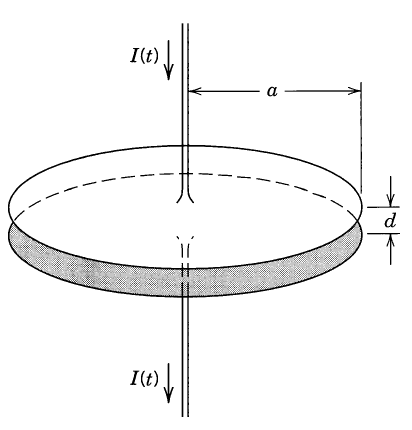
\includegraphics[scale=0.5]{problema3fig1}
\end{figure}

\begin{enumerate}[label=\textbf{(\alph*)}]
\item Calcule el campo eléctrico y el magnético entre las placas a segundo orden 
en potencias de la frecuencia (o número de onda), despreciado los efectos de campos 
de borde.
\item Calcule las integrales de volumen de $w_e$ y $w_m$ que entran en la definición 
de la reactancia $X$, (6.140), a segundo orden en $\omega$. Muestre que en términos 
de la corriente de entrada $I_i$, definida por $I_i = - i\omega Q$, donde $Q$ es 
a la carga total en una placa, estas energías son 

$$
\int w_e d^3x = \frac{1}{4\pi\epsilon}\frac{|I_i|^2d}{\omega^2 a^2}, \qquad 
\int w_m d^3x = \frac{\mu_0}{4\pi}\frac{|I_i|^2d}{8}\left(1 +
\frac{\omega^2 a^2}{12c^2} \right).
$$
\item Muestre que los circuitos en serie equivalentes tienen $C \simeq \pi\epsilon_0 
a^2/d$, $L \simeq \mu_0d/8\pi$, y que un estimado para la frecuencia de resonancia 
del sistema es $\omega_{res} \simeq 2\sqrt{2}c/a$. Compare con la primera raíz 
de $J_0(x)$.
\end{enumerate}

\vspace{.3cm}

\underline{Solución:} \vspace{.3cm}

\textbf{(a)} Por la simetría del problema trabajaremos en coordenadas cilíndricas polares $(\rho,\theta)$,
y por la forma de la corriente podemos asumir una dependencia temporal armónica 
para todas las cantidades. Si, como dice el enunciado, despreciamos los efectos 
de bordes, el sistema es simétrico en $\theta$, y el campo eléctrico entre las 
placas será en la dirección de $z$, mientras que el campo magnético irá en 
la dirección de la $\theta$. Podemos utilizar entonces las ecuaciones de Maxwell 
para campos armónicos\footnote{Ver ecuación (6.130) de Jackson \cite{jackson}.}, 
que tomando en cuenta las simetrías que acabamos de mencionar queda como 

\begin{equation}
 [\pmb{\nabla} \times \mathbf{E}]_\theta = - \frac{\partial E_z}{\partial \rho} = 
 i\omega B_\theta,
\end{equation}

\begin{equation}
 [\pmb{\nabla} \times \mathbf{B}]_z = \frac{1}{\rho}
 \frac{\partial (\rho B_\theta)} {\partial \rho} = - i\frac{\omega}{c^2}E_z,
\end{equation}

y ahora sustituyendo de la primera ecuación a la segunda obtenemos 

\begin{equation}
 \frac{d^2E_z}{d\rho^2} + \frac{1}{\rho}\frac{dE_z}{d\rho} + k^2E_z = 0,
\end{equation}

donde $k^2 = \omega^2/c^2$. Recordando la teoría de ecuaciones diferenciales y 
funciones especiales, vemos que esta es la ecuación de Bessel, la cual tiene 
una solución regular en $\rho=0$ igual a 

\begin{equation}
 E_z(\rho) ) = AJ_0(k\rho),
\end{equation}

donde $J_\alpha$ son las funciones de Bessel de primer tipo y $A$ es una constante 
a determinar. Por otra parte el campo magnético será 

\begin{equation}
 B_\theta(\rho) = \frac{i}{kc}\frac{dE_z}{d\rho} = - \frac{i}{c}AJ_1(k\rho).
\end{equation}

Para determinar la forma de $A$ utilizamos la ecuación para la densidad de 
carga superficial 

\begin{equation}
 \sigma(\rho) = \epsilon_0E_z(\rho) = \epsilon_0 A J_0(k\rho),
\end{equation}

e integrando encontramos que la carga total en la placa es 

\begin{equation}
 Q = 2\pi\epsilon_0A \int_0^a \rho J_0(k\rho) d\rho = 2\pi\epsilon_0\frac{a}{k} 
 AJ_1(ka).
\end{equation}

Resolviendo para $A$, relacionada a la carga $Q = iI_i/\omega$, encontramos 

\begin{equation}
 A = \frac{kQ}{2\pi a \epsilon_0 J_1(ka)}.
\end{equation}

Por lo tanto 

\begin{equation}
 E_z(\rho) = \frac{kQ}{2\pi a \epsilon_0 J_1(ka)} J_0(k\rho),
\end{equation}


\begin{equation}
 B_\theta(\rho) = - \frac{i}{c} \frac{kQ}{2\pi a \epsilon_0 J_1(ka)} J_1(k\rho).
\end{equation}

Entonces haciendo la expansión hasta segundo orden en $k$, utilizando relaciones 
para las funciones de Bessel\footnote{\href{http://bit.ly/1pslIha}{http://bit.ly/1pslIha}},
encontramos 

\begin{equation}
 \boxed{E_z(\rho) = \frac{Q}{\pi a^2 \epsilon_0}\left[1 + \left(\frac{a^2}{8} - \frac{\rho^2}{4}
 \right)k^2 + \dots \right]},
\end{equation}

\begin{equation}
 \boxed{B_\theta(\rho) = \frac{\mu_0I_i\rho}{2\pi a^2}\left[1 + \left(\frac{a^2}{8} - \frac{\rho^2}{4}
 \right)k^2 + \dots \right]},
\end{equation}

donde hemos usado $I_i = - i\omega Q$. 

\vspace{.3cm}

\textbf{(b)} Podemos ahora calcular las densidades armónicas de energía eléctrica 
y magnética, a segundo orden en $\omega$, que utilizando las ecuaciones (6.133) de 
Jackson \cite{jackson} podemos escribir como 

\begin{equation}
 \int w_e d^3x = \frac{\epsilon_0}{4}2\pi d \int_0^a \rho |E_z|^2 d\rho,
\end{equation}

\begin{equation}
 \int w_m d^3x = \frac{1}{4\mu_0}2\pi d \int_0^a \rho |B_\theta|^2 d\rho,
\end{equation}

e introduciendo estas integrales un poco complicadas en \texttt{Mathematica$^\circledR$}
encontramos que 

\begin{equation}
 \boxed{\int w_e d^3x = \frac{1}{4\pi\epsilon}\frac{|I_i|^2d}{\omega^2 a^2}},
\end{equation}

\begin{equation}
 \boxed{\int w_m d^3x = \frac{\mu_0}{4\pi}\frac{|I_i|^2d}{8}\left(1 +
\frac{\omega^2 a^2}{12c^2} \right)}.
\end{equation}

\hspace{10cm}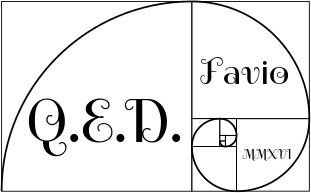
\includegraphics[scale=0.25]{logoQED}

\textbf{(c)} De la ecuación (6.140) de Jackson \cite{jackson} vemos que 

\begin{equation}
 X \simeq \frac{4\omega}{|I_i|^2}\int_V (w_m - w_e)d^3x,
\end{equation}

y sustituyendo las ecuaciones que encontramos en el inciso anterior tenemos que 

\begin{equation}
 X \simeq  \frac{\omega \mu_0 d}{8\pi} - \frac{d}{\epsilon_0 \omega \pi a^2},
\end{equation}

pero según el último párrafo de la sección 6.9 de Jackson \cite{jackson} (página 
267) también tenemos que 

\begin{equation}
 X \simeq \omega L - \frac{1}{\omega C},
\end{equation}

donde $L$ es la inductancia, y $C$ es la capacitancia. Igualando tenemos que 

\begin{equation}
 X \simeq \frac{\omega \mu_0 d}{8\pi} - \frac{d}{\epsilon_0 \omega \pi a^2} \simeq 
 \omega L - \frac{1}{\omega C},
\end{equation}

por lo tanto 

\begin{equation}
 \boxed{C \simeq \frac{\epsilon_0\pi a^2}{d}},
\end{equation}

\begin{equation}
 \boxed{L \simeq \frac{\mu_0d}{8\pi}}.
\end{equation}

Ahora recordando que la definición de la frecuencia de resonancia se define como 

\begin{equation}
 \omega_{res} \simeq \frac{1}{\sqrt{LC}} \simeq \sqrt{\frac{8}{\epsilon_0\mu_0 a^2}},
\end{equation}

podemos escribir entonces 

\begin{equation}
 \boxed{\therefore \omega_{res} \simeq \frac{2\sqrt{2}c}{a}}.
\end{equation}

\hspace{10cm}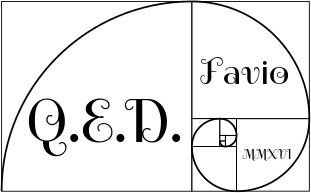
\includegraphics[scale=0.25]{logoQED}

Ahora $\frac{2\sqrt{2}c}{a} = 2.828 c/a$, y comparándola con $J_0 = 2.405$ vemos que 
si la razón $c/a$ es tal que al multiplicarla por $2.828$ nos de $2.405$, entonces 
la frecuencia de resonancia del sistema coincidiría con $J_0$.

\newpage

\begin{thebibliography}{10}
\bibitem{jackson}
J. Jackson, \emph{Classical Electrodynamics}, 3ra edición. John Wiley and Sons, Inc. 
1999.
\bibitem{griffiths}
D. Griffiths, \emph{Indtroduction to Electrodynamics}, 4ta edición. Pearson, 2013.
\end{thebibliography}

\end{document}